%%%%%%%%%%% Aquí va la solución al problema 4.
\newpage
\textbf{\textcolor{MidnightBlue}{4.}} Da una ejecución del algoritmo 3 para $n=4$ procesos y $t=1$ fallas bizantinas, en la que los procesos correctos no llegue a un consenso, a pesar de que los cuatro procesos, íncluido el Bizantino, empiecen con la misma propuesta y el bizantino sea el último de los coordinadores de la ejecución. Explica tu respuesta.
\begin{figure}
  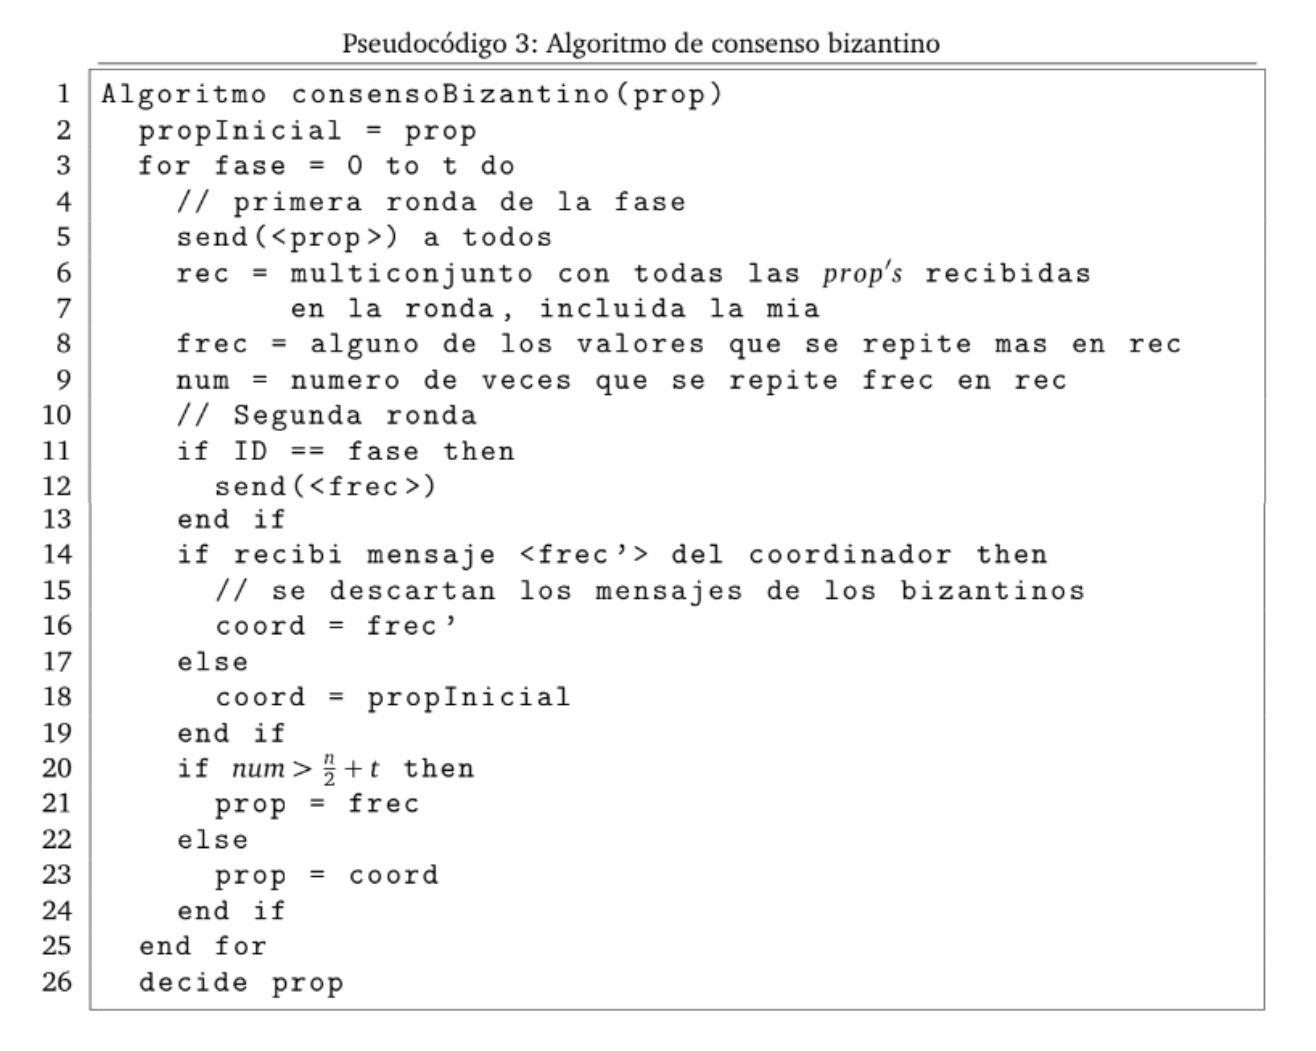
\includegraphics[width=\textwidth]{consensoBizantino.png}
\end{figure}